\chapter{ENTORNO EMPRESARIAL}

\section{Descripción de la empresa}
\subsection{Reseña histórica y actividad económica}
Donna S.A.C, una exitosa empresa dedicada a los minimercados, se ha establecido como un destino de compras esencial para la comunidad. Con cuatro ubicaciones estratégicas, esta cadena se ha convertido en un punto de referencia para aquellos que buscan productos de calidad y atención personalizada. Su lema, "Donna S.A.C, donde cada compra es una experiencia", refleja su compromiso con la creación de un ambiente cálido y acogedor para sus clientes. Desde la entrada, los clientes son recibidos con un diseño moderno y limpio, facilitando una experiencia de compra placentera. La atención al cliente es primordial, con empleados capacitados siempre dispuestos a brindar ayuda, garantizando que cada visita sea positiva.
\newline

Las cuatro tiendas de Donna S.A.C están estratégicamente ubicadas para ofrecer fácil acceso a una amplia gama de productos, desde alimentos frescos hasta artículos para el hogar, satisfaciendo las cambiantes necesidades de sus clientes. Con un equipo de veinte empleados comprometidos, Donna S.A.C ha cultivado un ambiente laboral colaborativo y motivador mediante una capacitación continua que asegura un servicio informado y útil para los clientes. Esta dedicación al desarrollo del equipo no solo beneficia a los empleados, sino que también contribuye al ambiente positivo que caracteriza a cada tienda.

\subsection{Descripción de la organización}

% Descripción de Donna S.A.C: Más Allá de un Minimarket, una Experiencia de Compra Inigualable.
% \newline

Donna S.A.C, una cadena de minimarkets que va más allá de las expectativas convencionales, ha dejado una marca distintiva en el mundo de las compras minoristas. Con cuatro ubicaciones estratégicas, esta empresa se ha convertido en un pilar esencial para aquellos que buscan no solo productos de elevada calidad, así mismo una experiencia de compra inigualable.
\newline

Cada tienda Donna S.A.C ha sido diseñada con esmero para crear un ambiente acogedor y moderno. Desde la entrada, los clientes son recibidos con un diseño limpio y una disposición intuitiva de productos. La tienda no es solo un espacio de transacciones; es un destino donde la atención al cliente es una prioridad. Nuestro equipo de veinte empleados capacitados está siempre disponible para ayudar, proporcionando un servicio personalizado que transforma cada visita en una experiencia positiva.
La diversidad de productos en Donna Sac es impresionante, desde alimentos frescos y productos del hogar hasta opciones de conveniencia para satisfacer las necesidades diarias. La cadena se enorgullece de mantener sus estantes abastecidos con productos de alta calidad, ofreciendo a los clientes la confianza de que encontrarán lo que necesitan, cuando lo necesiten.
\newline

Detrás de la exitosa operación de Donna Sac se encuentra un equipo de veinte trabajadores dedicados que personifican los valores de la empresa. La capacitación frecuente y el desarrollo profesional son fundamentales para nuestro enfoque en el servicio al cliente, asegurando que cada miembro del equipo esté bien informado y preparado para brindar asesoramiento útil.

\subsubsection{Organigrama}
Este organigrama es una representación simplificada de la estructura jerárquica de Donna Sac. Cada posición puede tener roles específicos y responsabilidades detalladas, y la organización está diseñada para fomentar la eficiencia operativa, la atención al cliente excepcional y la participación comunitaria.

\begin{figure}[h]
	\begin{center}
			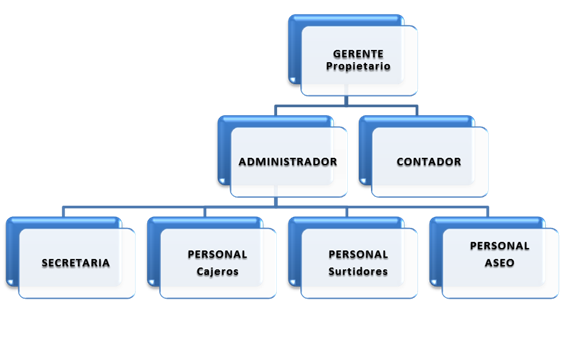
\includegraphics[width=0.8\textwidth]{31/figures/organigrama.png}
			\caption{Organigrama Donna SAC}
			\label{fig1}
	\end{center}			
\end{figure}

\subsection{Datos generales estratégicos de la empresa}
Información Básica:

\begin{itemize}
		\item Nombre completo de la empresa: Donna Sac.
		\item Fecha de fundación: 2000.
		\item Fundadores o actuales propietarios: Donaciano Paucar. 
		\item Tiendas: 6 tiendas.
		\item Ubicación de cada tienda: 2 en Chorrillos, Surco, 2 en La Molina, Breña.
		\item Tamaño promedio de las tiendas en pies cuadrados: 120 ft$^2$
		\item Número total de empleados: 40.
		\item Productos y Servicios: Consumo masivo.
		\item Segmentos de mercado objetivo: Personas proximas a las tiendas de Donna SAC.
\end{itemize}

\subsubsection{Visión, misión y valores o principios}
\textbf{Visión:} ``Ser reconocidos como el referente líder en la experiencia de compra minorista, destacando por nuestra dedicación excepcional al cliente, la innovación en productos y servicios, y nuestro impacto positivo en las comunidades que servimos."
\newline

\textbf{Misión:} ``En Donna Sac, nos comprometemos a ofrecer a nuestros clientes una experiencia de compra única y satisfactoria, brindando productos de alta calidad, un servicio personalizado y contribuyendo activamente al bienestar de las comunidades locales. Nos esforzamos por ser un destino esencial para aquellos que buscan más que una simple transacción, buscando una conexión significativa con sus necesidades diarias y valores compartidos."

\subsubsection{Objetivos estratégicos}
\textbf{Excelencia en la Experiencia del Cliente:}
\begin{itemize}
	\item Mejorar continuamente la atención al cliente para garantizar una experiencia de compra excepcional.
	\item Implementar programas de capacitación para el equipo humano que refuercen la significación del servicio al cliente.
\end{itemize}

\textbf{Diversificación y Ampliación de Productos:}
\begin{itemize}
	\item Investigar y agregar nuevos productos que satisfagan las tendencias del mercado y las necesidades cambiantes de los clientes.
	\item Expandir las líneas de productos propios para aumentar la diferenciación en el mercado.
\end{itemize}

\textbf{Innovación en Tecnología y Operaciones:}
\begin{itemize}
	\item Implementar tecnologías avanzadas para mejorar la eficiencia operativa, desde sistemas de gestión de inventario hasta soluciones de punto de venta.
	\item Explorar oportunidades para la implementación de plataformas digitales que mejoren la experiencia del cliente y faciliten la expansión en línea.
\end{itemize}

\textbf{Desarrollo de la Cadena de Suministro Sostenible:}
\begin{itemize}
	\item Contribuir con proveedores implicados con prácticas sostenibles y éticas.
	\item Reducir la huella ambiental mediante prácticas de gestión de residuos y opciones de embalaje sostenibles.
\end{itemize}

\textbf{Expansión Geográfica y Nuevas Tiendas:}
\begin{itemize}
	\item Identificar y evaluar nuevas ubicaciones estratégicas para la apertura de tiendas.
	\item Establecer alianzas con desarrolladores inmobiliarios para facilitar la expansión.
	\item Iniciativas de Responsabilidad Social Corporativa.
	\item Introducir iniciativas de responsabilidad social corporativa  
	\item Establecer asociaciones con organizaciones benéficas y participar activamente en eventos comunitarios.
\end{itemize}

\textbf{Optimización Financiera:}
\begin{itemize}
	\item Mejorar la eficiencia financiera mediante la implementación de herramientas de análisis y seguimiento.
	\item Buscar oportunidades para mejorar los márgenes de beneficio sin afectar la calidad de los recursos y servicios.
\end{itemize}

\subsubsection{Evaluación interna y externa. FODA}


	
%%%%%%%%%%%%%%%%%%%%%%%%%%%%%%

\begin{longtable}{L{5cm} | C{2.5cm} | C{2.5cm} | C{2.5cm} }
	\hline
	%\rowcolor{Gainsboro!60}
	\rowcolor{Gray}
	\makecell{Oportunidades} & \makecell{Ponderación}  & \makecell{Clasificación} & \makecell{Puntuación}\\
	\hline
	\endhead
	El crecimiento de la clase	media peruana está generando una mayor demanda de productos y servicios de calidad. La tendencia de los peruanos se está centrando en la obtención de productos de manera más rápida y en menores	tiempos de espera. & 0.3 & 3 &0.90\\
	\hline
	El cambio en los hábitos de consumo, los nuevos consumidores buscan cuidar su salud por lo que buscan frutas al momento de entrar a una tienda minorista. & 0.05 & 3 & 0.15\\
	\hline
	Cada vez salen nuevas marcas de productos de consumo masivo al mercado. Las alianzas estratégicas con otras empresas podrían ayudar a Donna a ampliar su oferta de productos. & 0.1 & 2 & 0.20\\
	\hline
	La innovación tecnológica podría ayudar a Donna  a mejorar la eficiencia y la experiencia de compra de los clientes. Implementación de IA en la capacitación o cajeros automáticos. & 0.05 & 2 & 0.10\\
	\hline
	Las inversiones en marketing podrían ayudar a Donna el aumentar su reconocimiento de marca y atraer a nuevos clientes. Expansión de sus redes sociales y crear campañas que se alineen con las nuevas tendencias en su público objetivo. & 0.15 & 1 & 0.15\\
	\hline
	 & 0.65 &  & 1.50\\
	\hline
	\caption{Oportunidades de Donna Sac}
	\label{tab:widgets}
\end{longtable}

%%AMENAZAS

\begin{longtable}{L{5cm} | C{2.5cm} | C{2.5cm} | C{2.5cm} }
	\hline
	%\rowcolor{Gainsboro!60}
	\rowcolor{Gray}
	\makecell{Amenazas} & \makecell{Ponderación}  & \makecell{Clasificación} & \makecell{Puntuación}\\
	\hline
	\endhead
	El crecimiento del sector de las tiendas minoristas está generando una mayor competencia. & 0.15 & 2 &0.30\\
	\hline
	Los cambios en la inestabilidad económica y cambios de gobierno reducen el tiempo de compra de productos. Muchos consumidores obtan por las tiendas mayoristas en este tipo de situaciones. & 0.05 & 2 & 0.10\\
	\hline
	Tambo posee una participación del 30\% en la categoria de tiendas minoristas. & 0.05 & 2 & 0.10\\
	\hline
	Los cambios en los hábitos de consumo, hacia una mayor orientación hacia los productos orgánicos o saludables, podrían afectar la demanda de los productos de Donna y replantear un nuevo stock de productos. & 0.05 & 3 & 0.15\\
	\hline
	Problemas de politica exterior de Perú con países a los que compramos productos internacionales podrian afectar el precio compra al que llegan a nuestro país. & 0.05 & 2 & 0.10\\
	\hline
	& 0.35 &  & 0.75\\
	\hline
	\caption{Amenazas de Donna Sac}
	\label{tab:widgets}
\end{longtable}

La empresa Donna se encuentra por debajo del promedio en cuestión de respuesta a los factores exteriores. Se recomienda darle más importancia a lo que esta pasando en su entorno macro para poder aprovechar las oportunidades del mercado.

\begin{longtable}{L{5cm} | C{2.5cm} | C{2.5cm} | C{2.5cm} }
	\hline
	%\rowcolor{Gainsboro!60}
	\rowcolor{Gray}
	\makecell{Fortalezas} & \makecell{Ponderación}  & \makecell{Clasificación} & \makecell{Puntuación}\\
	\hline
	\endhead
	Experiencia de 20 años en el mercado minorista, conocimientos del entorno y adaptación a los diversos escenarios del proceso de compra del consumidor. & 0.20 & 4 &0.80\\
	\hline
	Ofrece productos mucho más variados que otras tiendas minoristas que estan top en la categoría, Donna ofrece productos que abarcan hasta frutas y verduras que son del día. & 0.10 & 4 & 0.40\\
	\hline
	Donna se ubica en zonas de alto tráfico peatonal, lo que facilita el acceso a nuevos clientes & 0.05 & 3 & 0.15\\
	\hline
	Se ofrece una pequeña capacitación de unos 3 días al personal para que se enfoque en crear relación con el cliente y que no solo se convierta en una transacción de bienes. Se le proporciona videos y un taller que se enfoca en ser empatico con el cliente al preguntar cosas de su vida diaria. & 0.15 & 4 & 0.60\\
	\hline
	Empleados jóvenes, más agiles y que recomiendan productos a los clientes con mayor rapidez de acuerdo a las tendencias del mercado. & 0.10 & 3 & 0.30\\
	\hline
	& 0.60 &  & 2.25\\
	\hline
	\caption{Fortalezas de Donna Sac}
	\label{tab:widgets}
\end{longtable}

%%%%%DEBILIDADES

\begin{longtable}{L{5cm} | C{2.5cm} | C{2.5cm} | C{2.5cm} }
	\hline
	%\rowcolor{Gainsboro!60}
	\rowcolor{Gray}
	\makecell{Debilidades} & \makecell{Ponderación}  & \makecell{Clasificación} & \makecell{Puntuación}\\
	\hline
	\endhead
	La mayoría de las tiendas de Donna se encuentran en zonas urbanas, lo que limita su alcance al mercado rural. & 0.15 & 1 &0.15\\
	\hline
	Donna tiene una marca poco diferenciada, lo que puede dificultar su posicionamiento frente a la competencia que son en su mayoría tiendas de esquina o los mismos mercados. & 0.05 & 1 & 0.05\\
	\hline
	Donna se concentra en la venta de productos básicos, lo que limita su oferta de productos a un público más especializado. & 0.05 & 2 & 0.10\\
	\hline
	Donna no posee un horario de atención de 24 horas. & 0.10 & 1 & 0.10\\
	\hline
	Alta rotación de personal, no se crea identidad de marca con el personal interno. & 0.05 & 2 & 0.10\\
	\hline
	& 0.40 &  & 0.50\\
	\hline
	\caption{Debilidades de Donna Sac}
	\label{tab:widgets}
\end{longtable}


\begin{figure}[H]
	\begin{center}
		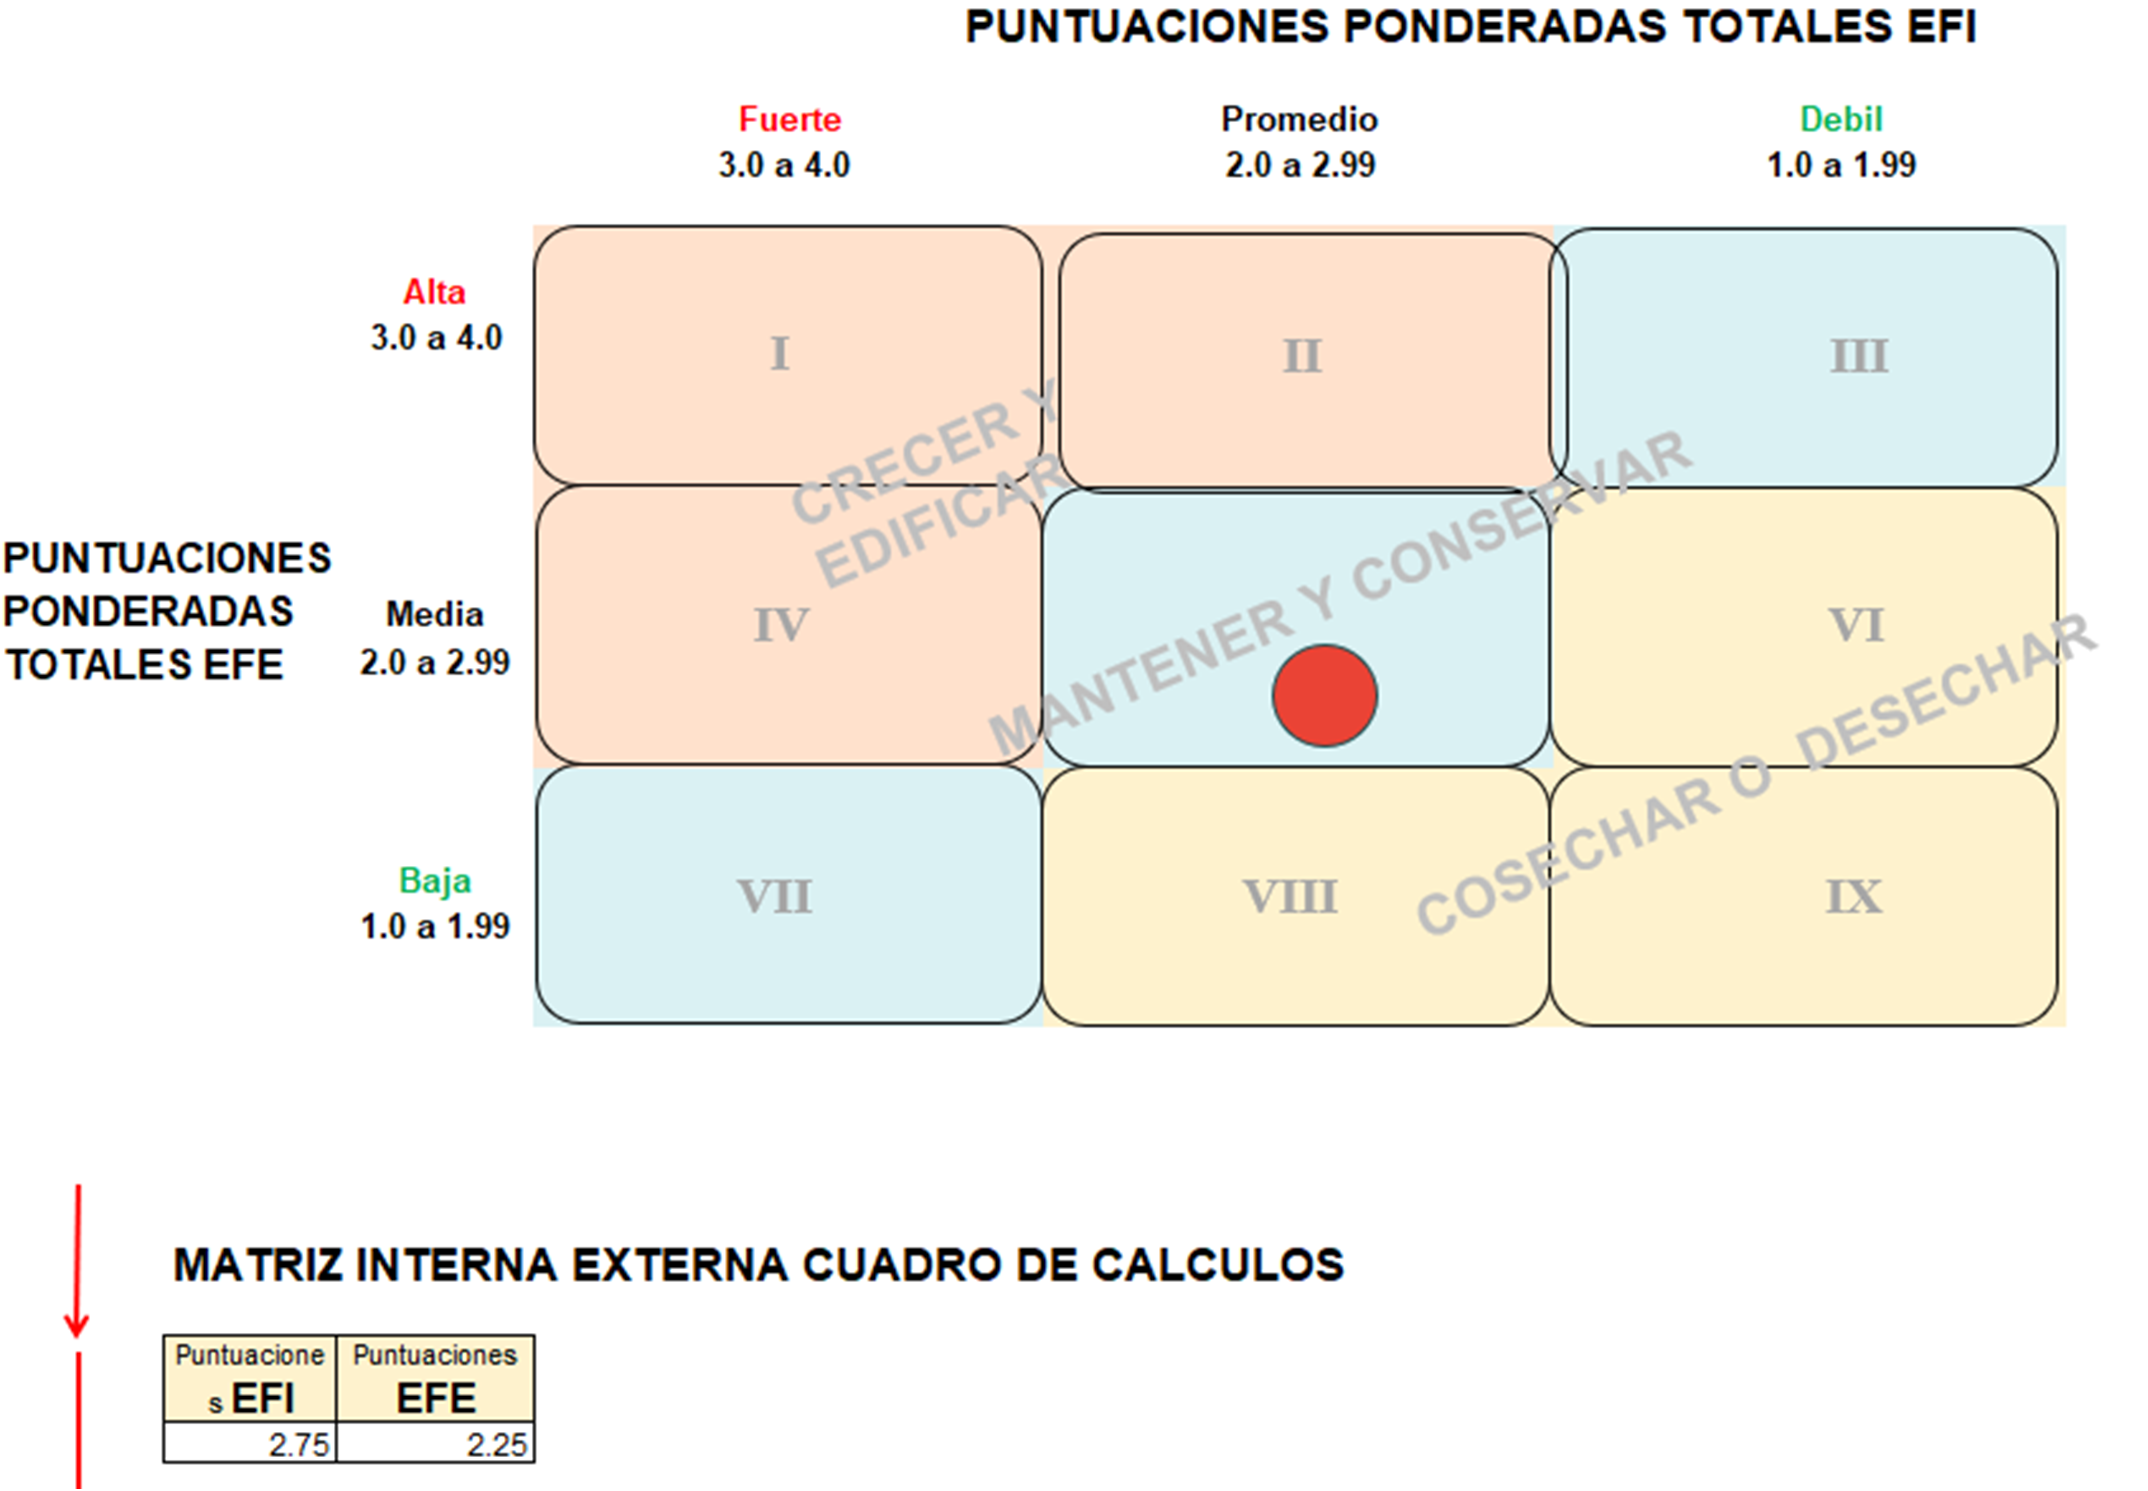
\includegraphics[width=0.8\textwidth]{31/figures/Matriz_EFI_EFE.png}
		\caption{Matriz interna y externa}
		\label{fig31.1}
	\end{center}			
\end{figure}

Donna se encuentra en la Celda V, por lo tanto le conviene la estrategia de mantener y conservar.  Lo que se plantea que haga Donna al no ser una opción la penetración de mercado por razones económicos es optar por la estrategia de desarrollo de producto. Lo que se plantea es introducir nuevos productos orgánicos y saludables, debido a la demanda de salud que está en crecimiento. Además, mejorar la calidad de productos y priorizar el bienestar del consumidor, darle un extra a cada compra para que pueda recordar nuestra marca.


\subsection{Modelo de negocio actual (CANVAS)}

\begin{figure}[H]
	\begin{center}
		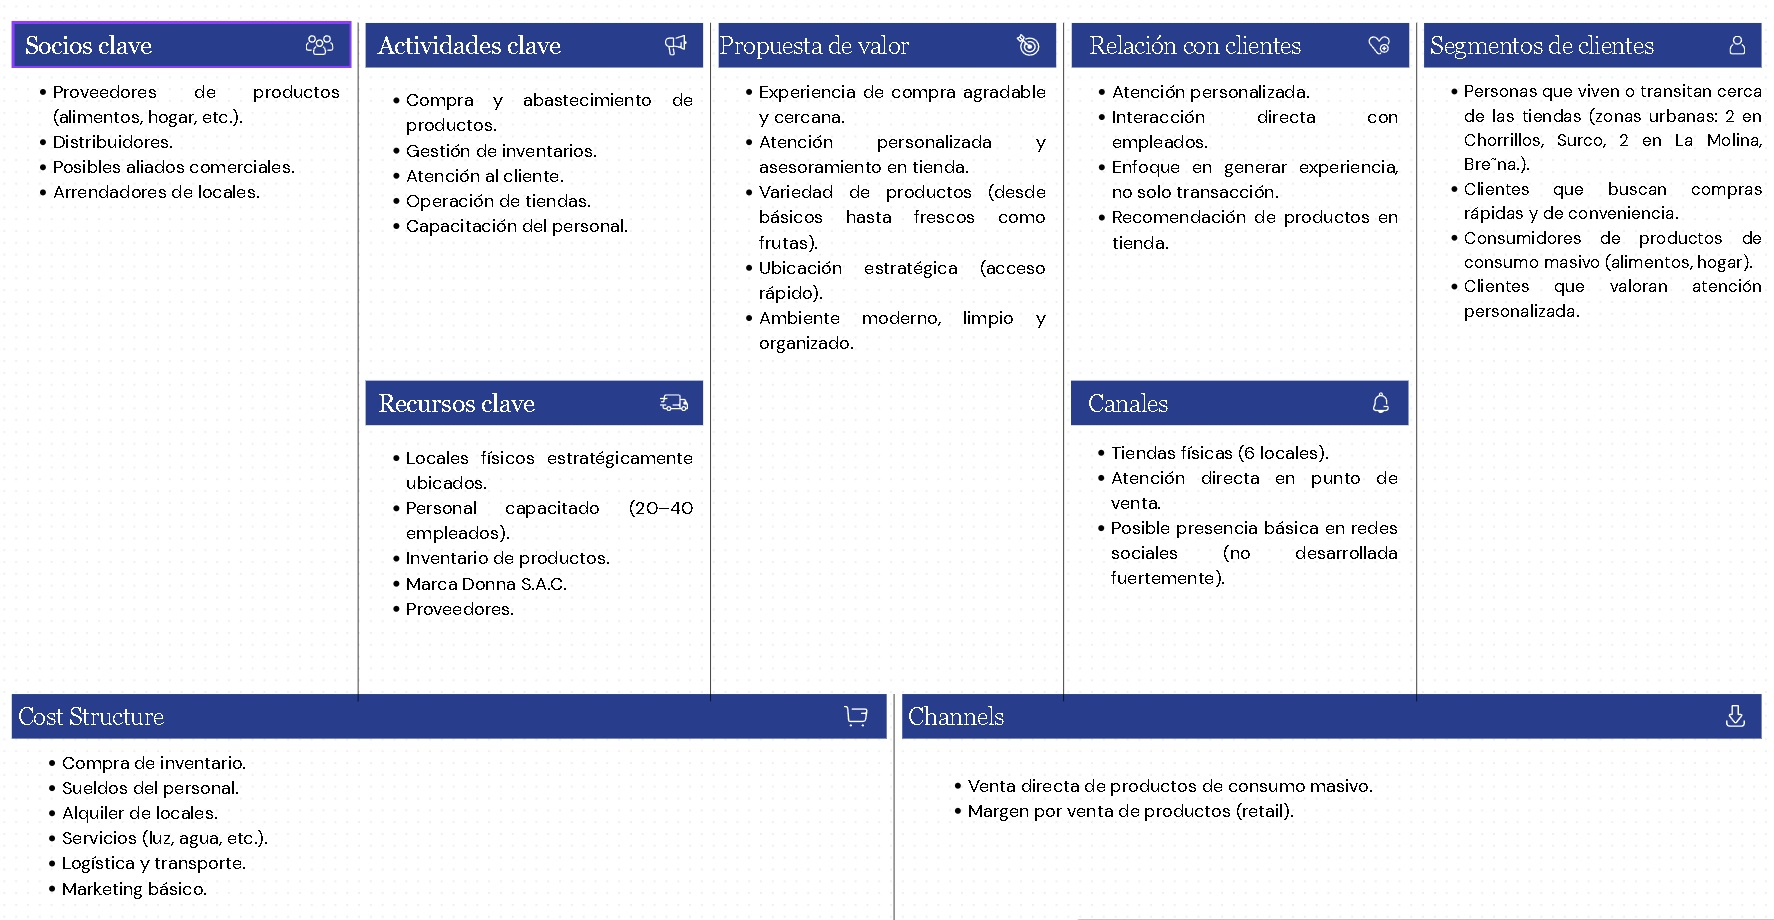
\includegraphics[width=0.9\textwidth]{31/figures/B CANVAS.JPG}
		\caption{Business Model Canvas}
		\label{fig31.2}
	\end{center}			
\end{figure}


% \subsection{Mapa de procesos actual}	



%\begin{longtable}{L{4cm} | C{2cm} | C{1.9cm} | C{1.9cm} | C{1.9cm} | C{1.9cm}| C{1.9cm}| C{1.9cm} }
%	\hline
%	%\rowcolor{Gainsboro!60}
%	\rowcolor{Gray}
%	\makecell{} & \makecell{} & \makecell{PERU} & \makecell{} & \makecell{COLOMBIA} & \makecell{} & \makecell{BRASIL}\\
%	\hline
%	\endhead
%		\makecell{Factores para el éxito} & \makecell{Ponderación}  & \makecell{Calificación} & \makecell{Puntuación} & \makecell{Calificación} & \makecell{Puntuación} & \makecell{Calificación} & \makecell{Puntuación}\\
%	\hline
%	
%	Crecimiento económico & 0.15 & 1 &0.15\\
%	\hline
%	Uso de Data Mining & 0.05 & 1 & 0.05\\
%	\hline
%	Expansión empresarial & 0.05 & 2 & 0.10\\
%	\hline
%	Desafíos en la gestión de inventarios & 0.10 & 1 & 0.10\\
%	\hline
%	Beneficios de la implementación de modelos predictivos & 0.05 & 2 & 0.10\\
%	\hline
%	Adopción de tecnologías emergentes & 0.40 &  & 0.50\\
%	\hline
%	Infraestructura logística & & & &\\
%	\hline
%	Participación en acuerdos comerciales & & & &\\
%	\hline
%	\caption{Debilidades de Donna Sac}
%	\label{tab:widgets}
%\end{longtable}




